\documentclass[12pt]{article}
%All the packages the project needs
%--------------------------------------------
%Margins
\usepackage[top=1.5cm,
bottom=2cm,
left=2.5cm,
right=2cm,
headsep=15pt,
headheight=25pt,
letterpaper,
includehead,includefoot]{geometry} 
%-------------------------------------------
%modification of paragraf for second title subsection
\usepackage{titlesec}
\setcounter{secnumdepth}{4}

\titleformat{\paragraph}
{\normalfont\normalsize\bfseries}{\theparagraph}{1em}{}
\titlespacing*{\paragraph}
{0pt}{3.25ex plus 1ex minus .2ex}{1.5ex plus .2ex}
%-------------------------------------------
%Codification and language
%Document language
\usepackage[spanish,es-noshorthands]{babel}
% Required for including letters with accents
\usepackage[utf8]{inputenc} 
% Use 8-bit encoding that has 256 glyphs
\usepackage[T1]{fontenc}
%-------------------------------------------

%-------------------------------------------
%Colours
\usepackage{color}
\usepackage{xcolor}
%-------------------------------------------

%-------------------------------------------
%Fonts and text
%Add a new Font
\usepackage{addfont}
\addfont{OT1}{rsfs10}{\rsfs}
%Allows to modify the font of a section
\usepackage{sectsty}
%Latin Modern fonts - Allows to resize the font
\usepackage{lmodern}
%Allows to write code
\usepackage{verbatim}
%Dumb text
\usepackage{lipsum}
%Include currency symbols
\usepackage{textcomp} 
%-------------------------------------------

%-------------------------------------------
%Pictures and graphics
%Allows to include images
\usepackage{graphicx}
\usepackage{sidecap}
%Most powerful image package
\usepackage{tikz}
\usetikzlibrary{babel}
\usetikzlibrary{positioning}
%Sometimes used images packages

\usepackage{pst-all}
\usepackage{pstricks}
%Allows to position figures inside a paragraph
\usepackage{wrapfig}
%Information needed
%https://en.wikibooks.org/wiki/LaTeX/Floats,_Figures_and_Captions
%-------------------------------------------
%-------------------------------------------
%Math packages
\usepackage{mathtools}
%\usepackage{unicode-math}
\usepackage{amsmath}
\usepackage{amssymb}
\usepackage{amsfonts}
%Nice cancelations arrows
\usepackage{cancel}
%Vector arrows on a character
\usepackage{esvect}
%-------------------------------------------

%-------------------------------------------
%Table and listing packages
\usepackage{multirow}
\usepackage{array}
\usepackage{diagbox}
\usepackage{listings}
\usepackage[shortlabels]{enumitem}
%\usepackage{table}
%Differents images and tables in the same space
\usepackage{subcaption}
%Use to places the float at precisely the location in the LaTeX code´and other stuff
\usepackage{float}
%Flexible tables
\usepackage{tabu}
\usepackage{multicol}
%-------------------------------------------

%-------------------------------------------
%Refs and cites
%\usepackage{achemso}
%\usepackage{natbib}
\usepackage{hyperref}
\usepackage[backend=biber,style=authoryear,citestyle=authoryear]{biblatex}
\hypersetup{
colorlinks=true,
urlcolor= blue,
citecolor=blue,
linkcolor= black,
bookmarks=true,
bookmarksopen=true,
}
\usepackage{csquotes}
\usepackage[backend=biber]{biblatex}
%\usepackage{cite}
%-------------------------------------------

%-------------------------------------------
%Boxes
\usepackage{tcolorbox}
\usepackage{fancybox}
\usepackage{colortbl}
%-------------------------------------------

%-------------------------------------------
%Page style
\usepackage[usestackEOL]{stackengine}
\usepackage{fancyhdr}
\pagestyle{fancy}
\newsavebox{\UNl}
\newsavebox{\UNd}
\setlength{\headheight}{2cm}
\renewcommand{\sectionmark}[1]{\markboth{\thesection\ #1}{}}
\renewcommand{\subsectionmark}[1]{\markright{\thesubsection\ #1}}
%\lhead{\usebox{\UNl}\usebox{\UNd}}
\lhead{\slshape \leftmark}
\rhead{\slshape \rightmark}
\cfoot{}
\rfoot{\thepage}
%\lfoot{\today}
\renewcommand{\headrulewidth}{1pt}

%-------------------------------------------

%-------------------------------------------
%others
\usepackage{pgfplots,caption}
\usepackage{comment}
\usepackage{pdflscape}
\usepackage{rotating}
\usepackage{parskip}
\usepackage{hhline}
\usepackage{longtable,lscape}
\usepackage{booktabs,bigstrut}
\usepackage{enumerate}
\usepackage{cleveref}
\usepackage{braket}
\usepackage{bigstrut}

\addbibresource{ref.bib}
\title{Proyecto de Tesis}
\author{Eduardo Andres Delgadillo Monsalve}
\date{\today}
%Inicio del documento
\pgfplotsset{compat=1.17}

\begin{document}
\renewcommand{\tablename}{Tabla}%% Para cambiar "Cuadro" a "Tabla"
\renewcommand{\listtablename}{Índice de tablas}
%Inicio de la portada
\begin{titlepage}
    \centering
    \thispagestyle{empty}
    \begin{center}
        \begin{figure}
        \centering%
        
\includegraphics{images/EscudoUN.png}
    \end{figure}
    
    \vspace{3cm}
    
    \textbf{CARACTERIZACIÓN DE LAS PROPIEDADES MORFOLÓGICAS, ÓPTICAS Y 
    TÉRMICAS DE LA REGOLITA PRESENTE EN LA SUPERFICIE LUNAR EN LA REGIÓN 
    DE LOS CRÁTERES GARAVITO}\\[1in]    
    Eduardo Andrés Delgadillo Monsalve \\  [3in]

   \textbf{Universidad Nacional de Colombia}\\
   Facultad de Ciencias\\
   Observatorio Astronómico Nacional\\
   Bogotá D.C.\\
   \today
    \end{center}
\end{titlepage}

\newpage
\begin{titlepage}
    \thispagestyle{empty}
    \begin{center}
        \begin{figure}
        \centering%
        
\includegraphics{images/EscudoUN.png}
    \end{figure}
    
    \vspace{1cm}
    
        \textbf{CARACTERIZACIÓN DE LAS PROPIEDADES MORFOLÓGICAS, ÓPTICAS Y 
        TÉRMICAS DE LA REGOLITA PRESENTE EN LA SUPERFICIE LUNAR EN LA REGIÓN 
        DE LOS CRÁTERES GARAVITO}\\[1in]    
    Eduardo Andrés Delgadillo Monsalve \\  [1.5 cm]
 Proyecto de tesis presentado como requisito parcial para optar al titulo de:\\[3mm]
 \textbf {\large{Magister en Ciencias Astronomia}}\\[1cm]
 Director:\\[3mm] PhD Mario Armando Higuera Garzón\\[1mm] 
 Observatorio Astronómico Nacional\\[1cm]
 Codirector:\\[3mm] PhD David Ardila\\ Jet Propulsion Laboratory\\[1in]
 \textbf{Universidad Nacional de Colombia}\\
 Facultad de Ciencias\\
 Observatorio Astronómico Nacional\\
 Bogotá D.C.\\
 \today
    \end{center}
\end{titlepage}
\newpage
\thispagestyle{empty}
\tableofcontents
\thispagestyle{empty}

\newpage
\listoffigures
\listoftables

\newpage
\setcounter{page}{1}
\section{Introducción}\label{sec:introduccion}
Desde siempre la observación de la Luna ha despertado un gran interés en la humanidad, 
las diferentes civilizaciones le han dado un significado especial y único, haciéndola parte 
de su cultura, sus relatos, sus mitos y creencias mas populares. Ha sido ese interés lo que 
en parte,  motivo a Galileo Galilei en el año de 1609 a observarla con su telescopio y 
publicar los primeros dibujos de la superficie lunar en su obra el Mensajero 
Sideral \parencite{galilei1610} y también lo que ha impulsado el desarrollo y 
conocimiento necesario para viajar a su superficie y colocar al primer ser humano en la Luna.\\
\\
En Colombia,el precursor de los estudios y de esa fascinación sobre la Luna, fue 
Julio Garavito Armero, que como director del Observatorio Astronómico Nacional en el año 1902 y 
como uno de los científicos Colombianos más importantes de su época, tuvo una gran 
impacto en el desarrollo de la ciencia, la astronomía y la ingeniería en Colombia. 
Sus estudios sobre ocultaciones de estrellas por la Luna y sobre las formulas definitivas 
para el calculo del movimiento de la Luna por el método de Hill Brown\parencite{GaravitoArmero_2017}, 
tuvieron relevancia tal, que el 27 de agosto de 1970 la Unión Astronómica Internacional (IAU) 
asigno el nombre de Garavito a un 
cráter de aproximadamente 80 kilómetros de ancho, en la cara oculta de la Luna. 
Dicho cráter se encuentra localizado en las coordenadas 47.6° de latitud Sur y 156.7° 
de longitud Este. Actualmente la región de Garavito en la Luna la componen cinco 
cráteres que llevan los nombres Garavito S, C, D, Q y Y.\\
\\
A lo largo del siglo pasado se desarrollaron las primeras misiones de exploración lunar, principalmente
los proyectos estadounidenses y soviéticos recopilaron información sobre el lado no visible  y sobre la 
superficie de la Luna \parencite{graf1993lunar}. En el presente mas países y agencias 
espaciales a nivel mundial se han unido a ese interés por la exploración Lunar, sobre todo por un 
inminente regreso de humanos a su superficie y al establecimiento de las primeras bases y colonias lunares. 
Las misiones que mas se destacan actualmente son las Chang'e de la Republica Popular de China y la 
Chandrayaan de la India, las cuales han recopilado los datos valioso sobre las principales características 
de la Luna. Por ejemplo la misión Chandrayaan realizo mediciones en el infrarrojo cercano, mediciones que 
permitieron detectar la presencia de agua en forma de Hielo en los polos de la Luna 
\parencite{VERMA2022115075}; 
la misión Chang'e-4 que es la primera misión con un rover en el lado no visible de la Luna,ha realizado 
mediciones con sus instrumentos para adquirir las curvas del espectro visible y el espectro infrarrojo 
\parencite{JIA2018207} \\
\\
El trabajo propuesto a continuación se centra en la caracterización, a partir de la información 
recopilada por las distintas sondas durante las misiones de exploración, especialmente las misiones Chang'e, 
que posee información del lado no visible, donde se ubican las regiones de 
los cráteres Garavito. Dicha caracterización investiga propiedades morfológicas, como relieve, tamaño, forma 
y composición de la regolita, también sus propiedades ópticas como reflectancia, albedo, 
condiciones de iluminación y sombra; y finalmente sus propiedades térmicas como la emisión 
en longitudes del infrarrojo\parencite{DSOUZA20242297}.

\newpage
\section{Objetivos}\label{sec:objetivos}
\subsection{Objetivo General}
Caracterizar las propiedades morfológicas, ópticas y térmicas de la regolita 
presente en los cráteres Garavito.
\subsection{Objetivos específicos}
\begin{itemize}
    \item Determinar los parámetros que definen la temperatura de la regolita 
    presente en la superficie lunar en la región de los cráteres Garavito\\    
    \item Reproducir las condiciones de radiancia solar que se observan sobre la 
    región de los cráteres Garavito durante un día lunar.\\    
    \item Establecer las curvas de emisión en las componentes ópticas y térmicas a 
    lo largo de un día lunar en la región de los cráteres Garavito.\\    
\end{itemize}

\newpage
\section{Planteamiento del problema}\label{sec:planteamiento}
La Luna posee ciertas características que la hacen particular, por ejemplo, su tamaño es bastante 
grande comparado con otras lunas del sistema solar de hecho se encuentra entre los satélites mas grandes
de los planetas conocidos \parencite{CarrascoLicea2021}, también el hecho de tener un acoplamiento de 
marea con la Tierra \parencite{Razmi_2005}. El acoplamiento de marea u 
orbita sincrónica significa que el periodo o el tiempo de rotación de la Luna sobre su 
propio eje es el mismo que el tiempo que tarda en completar una orbita alrededor de la 
Tierra. Este fenómeno se refleja en el hecho que, desde la tierra, siempre se observa 
la misma cara de la Luna. El lado no visible solo pudo ser observado por primera vez hasta 
el año de 1959, cuando la sonda espacial rusa, Luna 3, logro obtener la primera fotografía 
de ese lado oculto. Una imagen de las dos caras de la luna se presenta en la Figura \ref{fig:caras_luna}.
Esta necesidad de profundizar el conocimiento sobre las características morfológicas como  el relieve, 
topografía, material de la superficie, tamaños de las rocas 
y polvo lunar, del lado no visible, en especial de la región de los cráteres Garavito, 
es uno de los problemas que se buscan atender con los objetivos de este trabajo.
\\
\begin{figure}[H]
    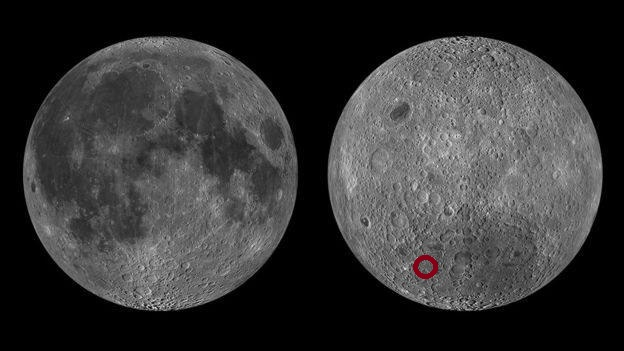
\includegraphics[width=0.7\textwidth]{images/Moon_sides.jpg}
    \centering
    \caption{Las dos caras de la Luna. Izquierda: el lado visible. Derecha: el lado 
    oculto. En rojo se muestra la ubicación de los Cráteres Garavito. 
    Fuente: NASA/GSFC/Arizona State University}
    \label{fig:caras_luna}
\end{figure}
Las condiciones y características que presenta el lado lejano de la Luna son muy diferentes 
a la cara cercana, por ejemplo en este lado se encuentra el cráter de impacto mas grande de la luna 
\parencite{LESLIE2019598} y en general suele suele ser mucho mas accidentada, por lo que posee un relieve 
mas irregular lo que influye, también, en las condiciones de 
iluminación de los cráteres, la cual esta dada principalmente por la acción del Sol, 
sin embargo, al igual que pasa en la tierra y debido a la inclinación del eje lunar respecto 
al plano de referencia horizontal (la eclíptica), la posición del sol en el cielo depende de la 
latitud  sobre la superficie, así entre mayor sea la latitud del 
observador más lejos estará el sol del cenit. Los parámetros principales para determinar  la 
posición del Sol en el cielo con la altura y el azimut, dos ángulos que se miden respecto 
al horizonte y respecto al norte, respectivamente\parencite{kolaczek1968selenocentric}. En la Figura 
\ref{fig:Altura_azimuth} se muestra 
La región que contiene los cráteres Garavito, con un azimut de 90°, lo que simularía una condición de 
iluminación desde el Este, y con diferentes alturas sobre el horizonte, se puede observar que 
las elevaciones y depresiones de la zona generan lugares que pueden estar más o menos 
expuestos a la incidencia de la radiación solar. Es necesario precisar este calculo durante el desarrollo 
del presente proyecto.\\
\begin{figure}[H]
    \centering
    \begin{subfigure}[b]{0.3\textwidth}
        \centering
        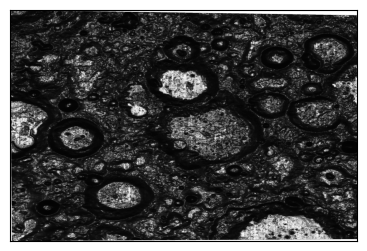
\includegraphics[width=\textwidth]{images/Azimuth_45_altitude_70.png}
        \caption{Altura:0 °}
        \label{fig: altura_70}
    \end{subfigure}
    \hfill
    \begin{subfigure}[b]{0.3\textwidth}
        \centering
        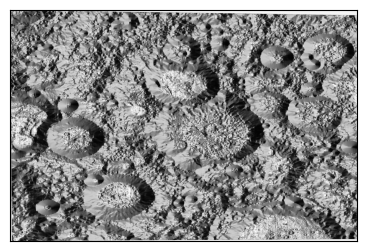
\includegraphics[width=\textwidth]{images/Azimuth_45_altitude_45.png}
        \caption{Altura : 30 °}
        \label{fig:altura_45}
    \end{subfigure}
    \hfill
    \begin{subfigure}[b]{0.3\textwidth}
        \centering
        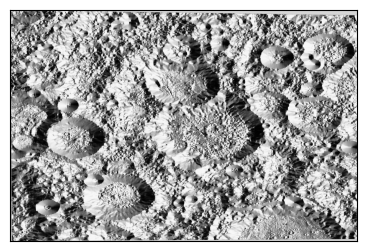
\includegraphics[width=\textwidth]{images/Azimuth_45_altitude_5.png}
        \caption{Altura : 60 °}
        \label{fig:altura_5}
    \end{subfigure}
    \caption{Mapa de sombras sobre la región de los cráteres Garavito, 
    a diferentes alturas del Sol. Fuente: elaboración propia con datos 
    del Lunar Orbiter Laser Altimeter(LOLA)}
    \label{fig:Altura_azimuth}
\end{figure}

El efecto que tiene la radiación sobre un cuerpo, es explicado por la teoría de la radiación 
del cuerpo negro, que describe el mecanismo por el cual un cuerpo absorbe o refleja la energía 
incidente sobre el \parencite{rybicki1991radiative}. Exceptuando las fuentes de radiación como estrellas, 
supernovas (SN), 
núcleos activos de galaxias (AGN), los rayos cósmicos, entre otros, cualquier objeto 
en el universo no es visible a no ser que algún tipo de radiación incida 
sobre él, por ejemplo si no existiera la luz incidente del sol sobre la Luna, esta seria imposible 
de ver. Alternativamente existe otra forma con la cual un objeto puede verse y es a través 
de emisión en el infrarrojo. \\
\\
La materia al ser impactada por energía, y absorber parte de esta, 
tiende a aumentar su temperatura. Esta relación entre entre la temperatura 
y la energía emitida por un cuerpo, se conoce como la ley de Stefan-Boltzmann,ecuación 
\ref{eq:Stefan–Boltzmann}\parencite{rybicki1991radiative}.
Por otra parte cualquier objeto que se encuentre por 
encima del cero absoluto (0 K), emite algún tipo de radiación, cuya longitud de onda va disminuyendo 
a media que aumenta de temperatura, es por eso que un metal al ser calentado pasar de ser rojo, a 
amarillo  y por ultimo a blanco. 
Para el caso de la Luna reconocer cómo el material de su superficie responde a esos cambios 
de temperatura es una tarea compleja por que responde a diferentes parámetros que controlan
dicha variación. Es por eso que definir y determinar las curvas de emisión es una tarea necesaria 
dentro de toda la caracterización de la zona de los cráteres Garavito.\\
\\
Identificar cómo todas estas características morfológicas vinculadas con las condiciones 
de iluminación y de incidencia de la radiación solar modifican la 
reflectancia y la emisión térmica de la superficie a lo largo de la duración del día lunar, es 
el objetivo principal de este trabajo.\\

\section{Antecedentes}
Aunque desde el siglo XX comenzó la exploración espacial de la Luna\parencite{nationalgeographic2024},
es en los últimos 20 años que se ha recobrado el interés por estudiar el lado no visible y se han 
desarrollado dispositivos que han hecho posible el alunizaje de nuevas misiones de 
exploración. La Tabla \ref{tab:misiones} muestra las principales misiones vigentes.\\
\\
Con base a esas primeras misiones que se enfocaron en la Luna, especialmente el proyecto Apolo de la 
Nasa y Luna de 
la Unión Soviética, se generó un catalogo del material 
de la superficie lunar. Dicho catalogo contiene la caracterización granulométrica y la 
distribución del tamaño de granos de las 143 muestras recolectadas en las misiones del Apolo 11, 12, 
14, 15, 16, 
y 17 y de la misión Luna 24, estos parámetros son básicos para una clasificación 
geológica y geotécnica, pues define las propiedades ópticas, térmicas, 
sísmicas, de esfuerzo y compresibilidad del suelo lunar \parencite{graf1993lunar}.\\
\begin{table}[H]
    \centering
    \caption{Misiones Vigentes sobre la Luna a Julio de 2023.}
    \begin{tabular}{|>{\centering\arraybackslash}m{13.07em}|>{\centering\arraybackslash}m{15.07em}|>{\centering\arraybackslash}m{10.145em}|}
        \toprule
        \textbf{Organización} & \textbf{Misión} & \textbf{Nombre} \\
        \midrule
        NASA - National Aeronautics and Space Administration & ARTEMIS (Acceleration, Reconnection, Turbulence and Electrodynamics of the Moon's Interaction with the Sun) & Themis B (ARTEMIS-P1) y Themis C (ARTEMIS-P2) \\
        \midrule
        NASA - National Aeronautics and Space Administration & Lunar Reconnaissance Orbiter & LRO \\
        \midrule
        ISRO - Indian Space Research Organisation & Chandrayaan & Chandrayaan-2 \\
        \midrule
        KARI - Korea Aerospace Research Institute & Korea Pathfinder Lunar Orbiter (KPLO) & Danuri \\
        \midrule
        NASA - National Aeronautics and Space Administration & Cislunar Autonomous Positioning System Technology Operations and Navigation Experiment & CAPSTONE \\
        \midrule
        JAXA - Japan Aerospace Exploration Agency & SELenological and ENgineering Explorer (SELENE) & KAGUYA (SELENE) \\
        \midrule
        CNSA - China National Space Administration & Chang'e 4 & Queqiao \\
        \bottomrule
    \end{tabular}
    \label{tab:misiones}
    \vspace{0.5em} \\
    \flushleft{*Elaborado a  partir de datos obtenidos de \cite{isro2024}}
\end{table}
Actualmente las sondas espaciales de la Nasa como el Lunar Orbiter Laser Altimeter (LOLA) y 
el satélite de retransmisión 
de datos de las misión Chang'e, el Queqiao, orbitan constantemente la luna.
Las distintas misiones, han recolectado una gran cantidad de datos a lo largo de los años en los que han 
estado activas. La misión LOLA por ejemplo ha producido modelos de gravedad lunar, modelos de brillo global, 
regional y local, mapas de pendientes y topográficos(Figura \ref{fig:elevacion_luna}). El LRO ha 
realizado medidas de radiación y ha generado la caracterización del ambiente de radiación Lunar global, 
también un modelo 3D de alta resolución (0.5 a 2 m/pixel) de la Luna y ha mapeado los tipos de roca 
y composición de suelos principales en la superficie Lunar. 
\begin{figure}[H]
    \includegraphics[width=0.7\textwidth]{images/Garavito_craters_LRO.png}
    \centering
    \caption{Elevación de los cráteres Garavito.
    Fuente: elaboración propia con datos del Lunar Orbiter Laser Altimeter(LOLA).}
    \label{fig:elevacion_luna}
\end{figure}
La misión Chandrayaan tiene instrumentos como el Moon Mineralogy Mapper o M3, para la medición en 
visible, infrarrojo cercano, rayos x de baja y alta energía, de los componentes químicos y mineralógicos de 
la superficie, además también tiene como objetivo ampliar el conocimiento de las características termo físicas 
y de la Luna. Por su lado La misión Chang'e 4 es la única que actualmente posee un rover operativo, 
el Yutu-2, que explora el lado lejano de la Luna. Entre los instrumentos de esta misión se destacan la 
cámara panorámica, el espectrómetro de baja frecuencia de radio y el radar de penetración lunar. 
La misión también ha recolectado muestras recientes  de la superficie del lado lejano que es posible 
consultar y visualizar 
\parencite{ZHAO2023115766}.

\section{Estado del Arte}\label{sec:estado_del_arte}
\subsection{Formación de Sistemas Planetarios}\label{sec:Sistemas solares}
\begin{figure}[H]
    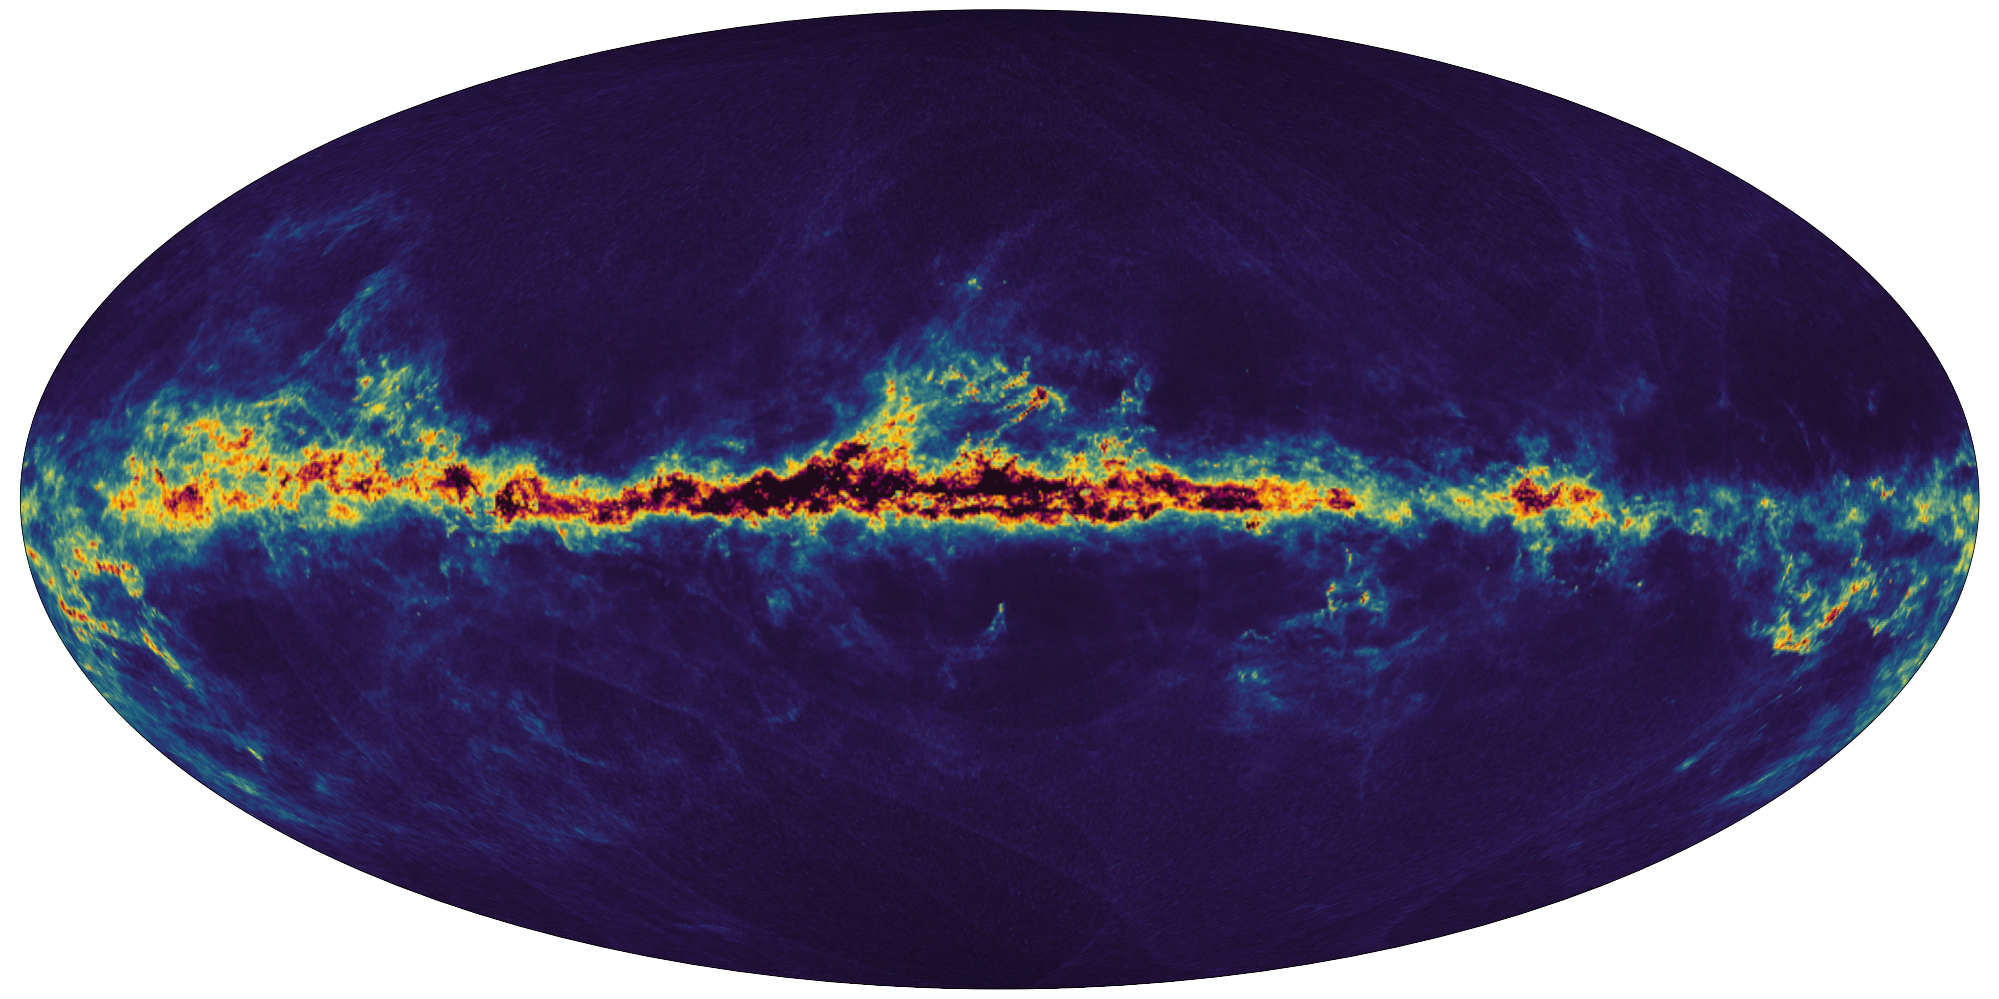
\includegraphics[width=0.7\textwidth]{images/Gaia_map_of_interstellar_dust_in_the_Milky_Way.png}
    \centering
    \caption{Mapa de la misión Gaia de polvo interestelar en la Vía Láctea. 
    Fuente: creado por T.E.Dharmawardena, Gaia group @ MPIA.}
    \label{fig:mapa_gaia}
\end{figure}
La evolución de las estrellas es un proceso muy complejo, una de las características mas importantes 
en ese proceso es el intercambio y la interacción con el material del entorno. El medio interestelar (ISM) 
no es un espacio vacío completamente sino que esta compuesto principalmente de gas y polvo, estos 
materiales inundan todo el espacio estelar extendiéndose al medio galáctico e incluso llegando 
a generar alguna interacción con el vecindario de galaxias mas cercanas a través de los vientos galácticos
\parencite{annurev:galacticwinds}. En la Figura \ref{fig:mapa_gaia} se muestra un mapa con la presencia 
de polvo en 
el medio interestelar de la Vía Láctea, las regiones mas oscuras representan una mayor cantidad de polvo 
esto se da principalmente hacia el centro de la galaxia y sobre el plano galáctico, las regiones en 
amarillo representan una menor cantidad de polvo que decrece hacia los bordes de la galaxia y las zonas 
azules y mas oscuras indican una menor cantidad de material, se puede notar también la presencia de polvo 
incluso mucho mas allá de los limites visibles de la misma galaxia.\\
\\
El polvo y el gas hacen parte fundamental en todo el ciclo estelar, existen regiones muy densas donde 
la acumulación de polvo y gas forma gigantes nubes, llamadas comúnmente nebulosas o nubes moleculares y 
que se conocen 
popularmente por ser la cuna de nacimiento de las estrellas. Es en esas nubes moleculares densas en donde 
se generan las condiciones necesarias para que la interacción de la temperatura, gas, polvo y gravedad 
se combinen para formar los primeros discos proto estelares y protoplanetarios.\\
\\
El proceso de la evolución estelar comienza  con la formación de las estrella es esas nubes de polvo y 
gas donde la acreción de material hace que la zona central colapse gravitacionalmente generando una 
proto estrella, luego a través de procesos termonucleares la estrella nace. A medida que estos procesos 
se incrementan también lo hacen la radiación, la temperatura y los vientos estelares. La evolución y 
vida de la estrella estar determinada principalmente por su masa y temperatura \parencite{Whittet2022DustIT}. 
De esa manera las estrellas mas masivas tendrán vidas mucho mas cortas que las estrella menos masivas. \\
\\
La evolución y clasificación de las estrellas se puede representar y visualizar fácilmente en el diagrama 
de Hertzsprung Russell o 
diagrama HR. El diagrama es esencialmente un grafico de la clase espectral/temperatura o color 
contrastado con el brillo de la estrella. La Figura \ref{fig:diagrama_HR} muestra el diagrama HR para un 
grupo grande de estrellas conocidas, incluyendo el propio Sol. 
Las clases espectrales se ubican de izquierda a derecha, la diagonal principal del diagrama contiene 
cerca del 80 \% de la estrellas y es llamada la secuencia principal, otros grupos se ubican arriba de 
la secuencia principal y son las estrellas llamas gigantes o supergigantes, y abajo de la secuencia 
principal se ubican las estrellas enanas blancas.
\begin{figure}[H]
    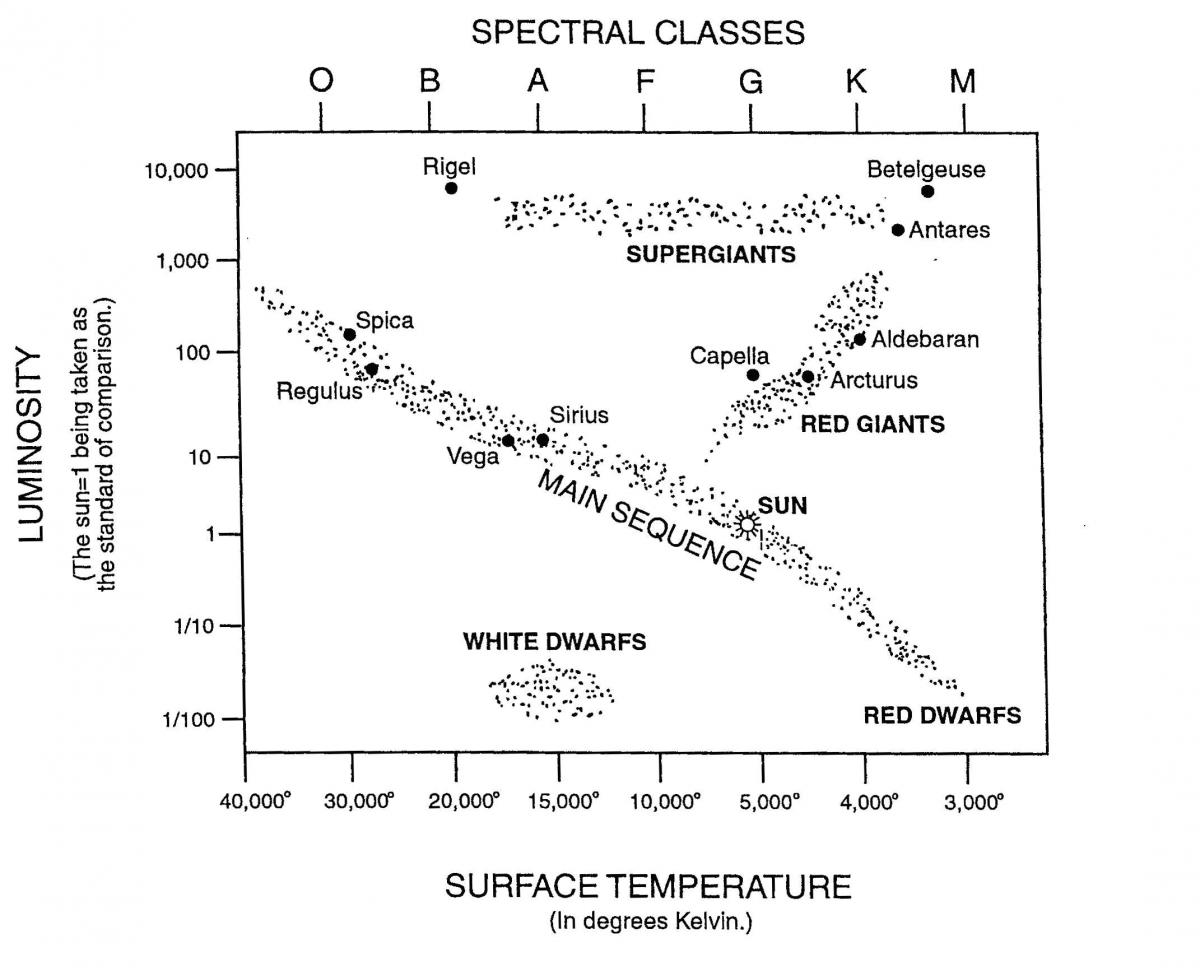
\includegraphics[width=0.6\textwidth]{images/HR_diagram.jpg}
    \centering
    \caption{Diagrama Hertzsprung-Russell con algunas estrellas conocidas. 
    Fuente: tomado de http://www.whitby-astronomers.com/focus/hertzsprung-russell-diagram.}
    \label{fig:diagrama_HR}
\end{figure}

\subsection{Origen del sistema solar}\label{sec:origen_solar}
Aunque no existe una evidencia directa sobre el proceso de formación del Sol, las observaciones en 
otras estrellas y el estudio de su ciclo han permitido establecer un escenario de origen del Sol a 
partir de una nube molecular primordial\parencite{TheFormationandEvolutionoftheSolarSystem}, dicha nube 
contenía los elementos esénciales para la formación del Sol y de los planetas del sistema solar actual. 
El sol es una estrella de tercera generación es decir que su composición contiene elementos que fueron 
formados en núcleos de estrellas anteriores, por lo menos hace dos generaciones de estrellas. Las 
primeras estrellas se formaron de los elementos mas abundantes del universo, hidrogeno y helio, estas 
estrellas y sus posteriores generaciones sintetizaron en sus núcleos los primeros elementos pesados, como 
el hierro y el aluminio, y por medio de sus muertes violentas inundarían el medio interestelar de estos 
elementos que serian utilizados para crear nuevas generaciones de estrellas. La estrella anterior al Sol 
ha sido llamada Coatlicue y se cree que era 30 veces mas masiva que el Sol. Esta teoría se refuerza con 
el hecho que metales mas pesados como el oro, la plata y el platino que se encuentra en la tierra, llegaron 
al entorno, mucho antes de la formación del Sol\parencite{Sun}.\\
\\
Y. Levin\parencite{levin2003origin}, menciona el colapso de la nube molecular que origino el sol dando 
paso a una proto estrella o proto Sol, y un disco de acreción protoplanetario compacto y giratorio. 
Esta nebulosa proto planetaria evoluciono acumulando polvo y roca en planetesimales. Estos objetos 
continuaron barriendo sus orbitas, acumulando materiales, colisionando entre ellos, para formar los 
primeros protoplanetas rocosos, con un núcleo metálico y un manto de silicatos, que se convertirían 
eventualmente en un sistema planetario.
\begin{figure}[H]
    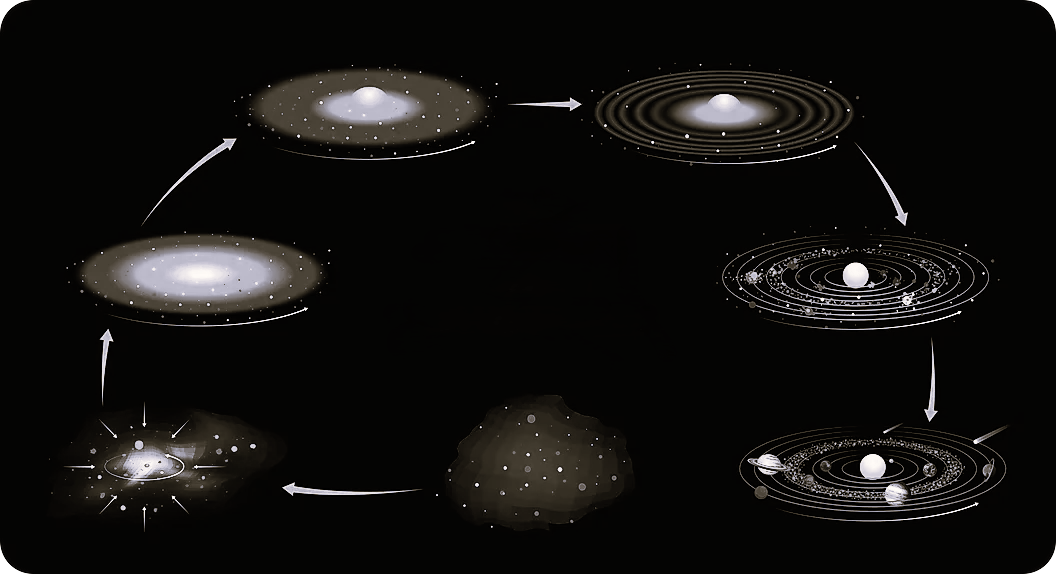
\includegraphics[width=0.7\textwidth]{images/System_solar_origin.png}
    \centering
    \caption{Diagrama representativo básico de la formación del sistema solar.
    Fuente: adaptado de https://www.worldatlas.com/space/the-origin-of-planet-earth.html}
    \label{fig:formation_solar_System}
\end{figure}

Las órbitas casi planas y casi circulares de los planetas en el sistema solar argumentan 
fuertemente a favor de la formación planetaria dentro de un disco circumsolar aplanado. Los modelos
astrofísicos sugieren que tales discos son un subproducto natural de la formación estelar a partir 
del colapso de núcleos rotativos de nubes moleculares. La evidencia observacional de la presencia
de discos de dimensiones del sistema solar alrededor de estrellas jóvenes ha aumentado sustancialmente 
en los últimos años, y los excesos infrarrojos en los espectros de estrellas jóvenes sugieren
que las vidas útiles de los discos protoplanetarios varían entre $10^6$ y $10^7$ años.

Nuestra galaxia contiene muchas nubes moleculares, la mayoría de las cuales son varios órdenes de 
magnitud más grandes que nuestro sistema solar. Las nubes moleculares son las partes más frías y
densas del medio interestelar. Son inhomogéneas, y las partes más densas de las nubes moleculares se 
denominan núcleos. Estos son los sitios en los que ocurre la formación estelar en la época actual.
Incluso un núcleo de nube molecular que rota muy lentamente tiene demasiado momento angular de giro 
para colapsar en un objeto de dimensiones estelares, por lo que una fracción significativa del
material en un núcleo en colapso cae sobre un disco orbital soportado por rotación alrededor de la 
(proto)estrella soportada por presión. Este disco tiene la misma composición elemental inicial que
la estrella en crecimiento. A distancias suficientemente grandes de la estrella central, es lo 
suficientemente frío como para que $\sim$1\%-2\% de este material esté en forma sólida, ya sea granos
interestelares remanentes o condensados formados dentro del disco. Este polvo está compuesto 
principalmente por compuestos formadores de rocas dentro de unos pocos UA de una estrella de 
1 M$\odot$, pero en las regiones más frías y distantes, la cantidad de hielos (por ejemplo, H$_2$O, 
CH$_4$, CO) presentes en forma sólida es comparable a la de los sólidos rocosos.

Durante las etapas iniciales, se presenta un fenomeno denominado infall, en la que el material en el disco 
circumstellar, principalmente gas y polvo, cae hacia el centro, en esta etapa el disco es muy activo y probablemente 
altamente turbulento como resultado de la discrepancia del momento angular específico del gas que golpea 
el disco con el requerido para
mantener la rotación kepleriana. Las inestabilidades gravitacionales y las fuerzas viscosas y magnéticas 
pueden sumarse a esta actividad. Cuando la infall disminuye sustancialmente o se detiene, el disco se
vuelve más tranquilo. Las interacciones con la componente gaseosa del disco afectan la dinámica de los 
cuerpos sólidos pequeños, y el crecimiento desde el polvo de tamaño micrométrico hasta los
planetesimales de tamaño kilométrico sigue siendo poco comprendido. Los meteoritos, los planetas menores 
y los cometas, la mayoría de los cuales nunca se incorporaron en cuerpos de dimensiones planetarias, 
conservan mejor un registro de este período importante en el desarrollo del sistema solar.

La dinámica de los cuerpos sólidos más grandes dentro de los discos protoplanetarios está mejor caracterizada. 
Las principales perturbaciones en las órbitas keplerianas de los planetesimales de tamaño kilométrico y más 
grande en los discos protoplanetarios son interacciones gravitacionales mutuas y colisiones físicas. Estas
interacciones conducen a la acreción (y en algunos casos erosión y fragmentación) de planetesimales. Eventualmente, 
los cuerpos sólidos se aglomeraron en los planetas terrestres en el interior del sistema solar y en núcleos 
planetarios varias veces la masa de la Tierra en el exterior del sistema solar. Estos núcleos masivos fueron capaces
de atraer y retener material gaseoso sustancial de la nebulosa solar. En contraste, los planetas terrestres no 
fueron lo suficientemente masivos como para atraer y retener tales gases, y los gases en sus
atmósferas delgadas actuales provienen del material que se incorporó en planetesimales sólidos.

Los planetas en nuestro sistema solar orbitan lo suficientemente cerca entre sí que las fases finales del 
crecimiento planetario podrían haber involucrado la fusión o expulsión de planetas o
embriones planetarios en órbitas inestables. Sin embargo, las bajas excentricidades de las órbitas de los 
planetas exteriores implican que algún proceso de amortiguación, como la acreción/expulsión de
numerosos pequeños planetesimales o interacciones con gas residual dentro del disco protoplanetario, 
también debe haber estado involucrado.

A medida que los investigadores aprenden más sobre los cuerpos individuales y las clases de objetos en 
nuestro sistema solar, y a medida que las simulaciones del crecimiento planetario se vuelven
más sofisticadas, las teorías sobre la formación de del sistema solar se están revisando y 
mejorando. La detección de planetas alrededor de otras estrellas  ha presentado nuevos 
desafíos para desarrollar una teoría unificada de la formación planetaria que sea más generalmente aplicable.
\parencite{PLanet_formation}.
\begin{itemize}
    \item Cuando un núcleo de nube molecular colapsa, la porción
    interna se convierte en una estrella. El material de la nube
    molecular con alto momento angular cae en un disco alrededor de
    esa estrella y está disponible para la formación planetaria.
    \item Mientras que los planetas crecen por acreción de cuerpos
    pequeños en cuerpos más grandes, las estrellas se forman mediante
    el colapso de grandes nubes en objetos más pequeños.
\end{itemize}

\subsection{Radiación del Cuerpo Negro y SED: Distribución Espectral de Energía}\label{sec:radiacion}
La radiación térmica es la radiación emitida por un cuerpo como consecuencia de su temperatura.
Todo los cuerpos emiten esta radiación a su alrededor, y la absorben de él. Si, en 
un principio el cuerpo esta mas caliente que su alrededor, se enfriara, ya que la rapidez con que emite 
energía excederá la rapidez con la que absorbe. Cuando  se alcanza el equilibrio térmico la 
rapidez de emisión y la de absorción de energía serán iguales.
Un aspecto importante de la radiación astrofísica es la interacción de la radiación con la materia a 
medida que la radiación se propaga a través de un medio. La descripción matemática de esta interacción 
está contenida en la ecuación de transferencia radiactiva.
\begin{figure}[H]
    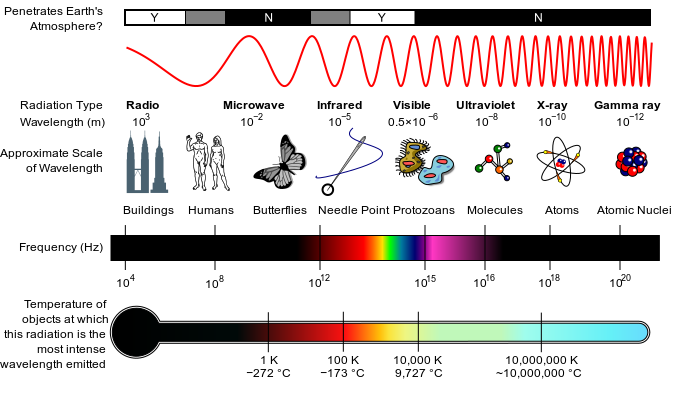
\includegraphics[width=0.7\textwidth]{images/EM_Spectrum_Properties_edit.png}
    \centering
    \caption{Emisión de todo el espectro electromagnético, con longitud de onda y frecuencia.
    Fuente: adaptado de https://commons.wikimedia.org/wiki/spectrum}
    \label{fig:spectrum_radiacion}
\end{figure}
La radiación electromagnética consiste en fotones en muchas longitudes de onda; un espectro de la 
emisión electromagnética se muestra en la Figura \ref{fig:spectrum_radiacion}. La frecuencia, $\nu$, 
de una onda electromagnética que se propaga en el vacío está relacionada con su longitud de onda, 
$\lambda$, por

\begin{equation}
    \lambda \nu = c,
    \label{eq:luz}
\end{equation}

donde $c$ es la velocidad de la luz en el vacío, $c = 2.998 \times 10^8$ m s$^{-1}$.\\
\\
La mayoría de los objetos emiten un espectro continuo de radiación electromagnética. Esta emisión térmica
se aproxima bien mediante la teoría de la radiación de cuerpo negro. Un cuerpo negro se define como un objeto
que absorbe toda la radiación que incide sobre él a todas las frecuencias y todos los ángulos de incidencia; 
es decir, no se refleja ni se dispersa radiación alguna. La capacidad de un cuerpo para emitir radiación es 
la misma que su capacidad de absorber radiación a la misma frecuencia. La radiación emitida por un cuerpo 
negro se describe mediante la ley de radiación de Planck.
\begin{equation}
    B_{\nu} (T) = \frac{2h\nu^3}{c^2} \frac{1}{e^{h\nu/(kT)} - 1},
    \label{eq:plank}
\end{equation}
donde $B_{\nu} (T)$ es la intensidad (W m$^{-2}$ Hz$^{-1}$ sr$^{-1}$) y $h$ es la constante de Planck. 
La Figura \ref{fig:curva_radiacion}a muestra un gráfico de la intensidad en función de la frecuencia 
para varios cuerpos negros con temperaturas que van desde 40 hasta 30 000 K. Un espectro de nuestro 
Sol se muestra en la Figura \ref{fig:curva_radiacion}b, con una curva de cuerpo negro superpuesta a 
una temperatura de 5777 K. Estas dos figuras muestran que la intensidad del Sol alcanza su máximo en 
longitudes de onda ópticas. En contraste, las de los planetas ($\sim$40–700 K) alcanzan su máximo en 
longitudes de onda infrarrojas. La intensidad de la mayoría de los objetos del sistema solar cerca de 
sus picos espectrales puede aproximarse bastante bien mediante curvas de cuerpo negro.\\
\\
Dos relaciones muy importantes pueden derivarse de la ley de radiación de Planck:
\subsubsection{Ley de Rayleigh–Jeans}

Cuando $h\nu \ll kT$ (es decir, en longitudes de onda de radio para temperaturas típicas de cuerpos planetarios), 
el término $(e^{h\nu/(kT)} - 1) \approx \frac{h\nu}{kT}$ y la ecuación \ref{eq:plank} se puede aproximar a:

\begin{equation}
    B_\nu (T) \approx \frac{2\nu^2 kT}{c^2}
    \label{eq:Rayleigh}
\end{equation}

\subsubsection{Ley de Wien's}
Cuando $h\nu \gg kT$:

\begin{equation}
    B_\nu (T) \approx \frac{2h\nu^3}{c^2} e^{-h\nu/(kT)}
    \label{eq:Wiens}
\end{equation}

Las ecuaciones \ref{eq:Rayleigh} y \ref{eq:Wiens} son más simples que la ecuación \ref{eq:plank}, y por lo tanto 
pueden ser bastante útiles en los regímenes en los que son aplicables.\\
\begin{figure}[H]
    \centering
    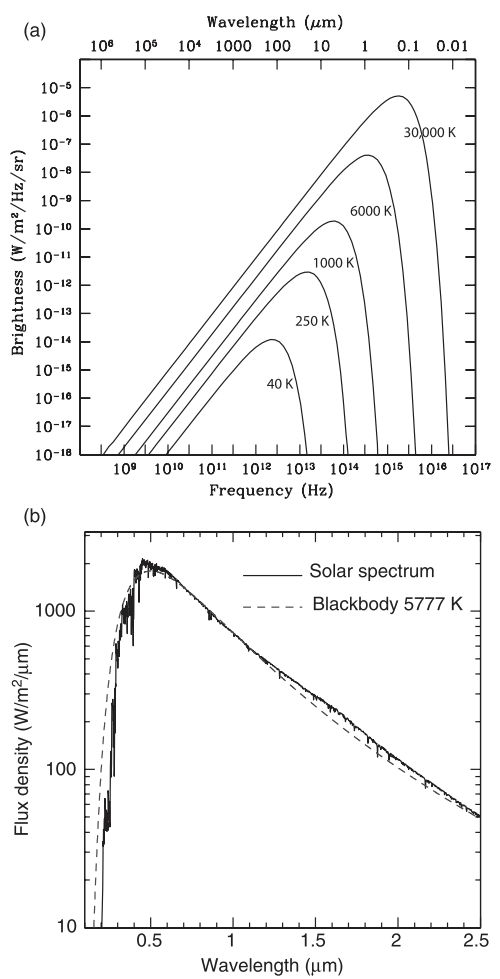
\includegraphics[width=0.4\textwidth]{images/waavelength.png}
    \caption{(a) Curva de radiación de un cuerpo negro como una función de la frecuencia, $\nu$.
    (b) Espectro de radiación del Sol como una función de la longitud de onda, $\lambda$, y la radiación de 
    un cuerpo negro con una temperatura de 5770 K. Fuente: tomado de Fundamental Planetary Science. Jack J. Lissauer}
    \label{fig:curva_radiacion}
\end{figure}

La frecuencia, $\nu_{\text{max}}$, en la que el pico de la intensidad, $B_\nu (T)$, ocurre puede determinarse 
estableciendo la derivada de la ecuación \ref{eq:plank} igual a cero, $\partial B_\nu / \partial \nu = 0$. 
El resultado es conocido como la ley de desplazamiento de Wien:

\begin{equation}
    \nu_{\text{max}} = 5.88 \times 10^{10} T
\end{equation}

con $\nu_{\text{max}}$ en Hz y T en grados Kelvin. Con $B_\lambda = B_\nu \frac{d\nu}{d\lambda}$, el pico espectral 
de un cuerpo negro en longitud de onda se puede encontrar estableciendo $\partial B_\lambda / \partial \lambda = 0$:

\begin{equation}
    \lambda_{\text{max}} = \frac{2.9 \times 10^{-3}}{T}
    \label{eq:desplazamiento_wiens}
\end{equation}

con $\lambda_{\text{max}}$ en fracciones de un metro y T en Kelvin. \\

\subsubsection{Ley de Stefan–Boltzmann}
La densidad de flujo, $F_\nu$ (W m$^{-2}$ Hz$^{-1}$), de la radiación de un objeto está dada por:

\begin{equation}
F_\nu = \Omega_s B_\nu (T)
\end{equation}

donde $\Omega_s$ es el ángulo sólido subtendido por el objeto. Justo por encima de la ‘superficie’ de un planeta con 
brillo $B_\nu$, la densidad de flujo es igual a:

\begin{equation}
F_\nu = \pi B_\nu (T)
\end{equation}

El flujo, $F$ (J s$^{-1}$ m$^{-2}$), se define como la densidad de flujo integrada sobre todas las frecuencias:

\begin{equation}
    F \equiv \int_0^\infty F_\nu d\nu = \pi \int_0^\infty B_\nu (T) d\nu = \sigma T^4
    \label{eq:Stefan–Boltzmann}
\end{equation}

donde $\sigma$ es la constante de Stefan–Boltzmann. La ecuación \ref{eq:Stefan–Boltzmann} es conocida como la ley de 
Stefan–Boltzmann.\\
\\
Los cuerpos planetarios se calientan principalmente al absorber radiación del Sol y pierden energía 
mediante la radiación al espacio. Mientras que un punto en la superficie de un cuerpo es iluminado por 
el Sol solo durante el día, irradia tanto de día como de noche. La cantidad de energía incidente por 
unidad de área depende tanto de la distancia al Sol 
como del ángulo de elevación local del Sol. Como consecuencia, la mayoría de los lugares son más fríos 
alrededor del amanecer y más calientes un poco después del mediodía local, y las regiones polares son 
(en promedio) más frías que el ecuador para cuerpos con una oblicuidad 
$\psi < 54^\circ$ (o $\psi > 126^\circ$) \parencite{PLanet_formation}.\\
\\
A largo plazo, la mayoría de los cuerpos planetarios irradian casi la misma cantidad de energía al 
espacio que la que absorben de la luz solar; si este no fuera el caso, los planetas se calentarían o 
enfriarían. (Los planetas gigantes Júpiter, Saturno y Neptuno son excepciones a esta regla. 
Estos cuerpos irradian significativamente más energía de la que absorben porque aún están perdiendo el 
calor producido durante el tiempo de su formación.) Aunque el equilibrio global a largo plazo es la norma, 
las fluctuaciones espaciales y temporales pueden ser grandes. La energía se almacena del día a la noche, 
del perihelio al afelio y del verano al invierno, y puede transportarse de un lugar a otro en un planeta.

\subsection{Albedo}
Cuando un objeto es iluminado por el Sol, refleja parte de la energía de vuelta al espacio (lo que hace
que el objeto sea visible para nosotros), mientras que la energía restante es absorbida. En principio, uno 
puede determinar cuánta de la radiación incidente es reflejada al espacio en cada frecuencia; la relación entre 
la energía incidente y la energía reflejada + dispersada se llama albedo monocromático, $A_\nu$. 
Integrando sobre la frecuencia, la relación de la radiación total reflejada o dispersada por el objeto a la 
luz total incidente del Sol se llama albedo de Bond, $A_b$. La energía o flujo absorbido por el objeto determina
su temperatura. También es importante considerar cómo una superficie dispersa la luz. La luz del Sol es dispersada por
un planeta y recibida por un telescopio.\\
\begin{figure}[H]
    \centering
    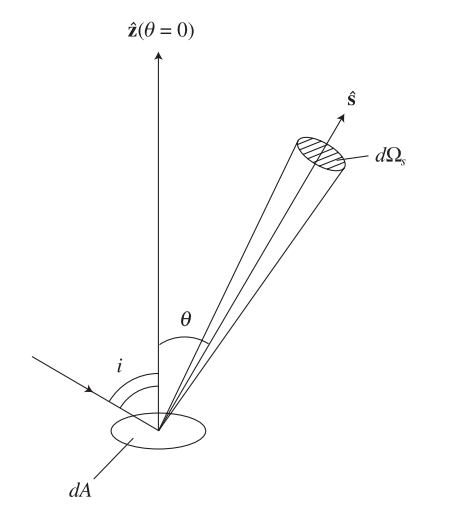
\includegraphics[width=0.4\textwidth]{images/diagrama_albedo.png}
    \caption{Diagrama de un elemento con superficie $\mathrm{d}A$, con un rayo incidente. 
    Fuente: tomado de Fundamental Planetary Science, Jack J. Lissauer.}
    \label{fig:diagrama_albedo}
\end{figure}
Los tres ángulos de relevancia se indican en las Figuras \ref{fig:diagrama_albedo} y
\ref{fig:albedo_Reflejo}: El ángulo que hace la luz incidente con la normal a la superficie del planeta, $i$, y 
el ángulo que
se refleja es recibido en el telescopio (es decir, el rayo a lo largo de la línea de visión) que forma con la 
normal a la superficie, $\theta$, se muestra en la Figura 4.3; el ángulo de fase o ángulo de reflectancia, $\phi$, 
visto desde el objeto se muestra en la Figura 4.4. Para la radiación puramente retro dispersada, el ángulo de fase 
$\phi = 0$; en el caso de la luz dispersada hacia adelante, $\phi = 180^\circ$. A menudo, la luz se dispersa en una 
dirección preferida, lo que puede expresarse mediante la función de fase de dispersión. En particular, para 
partículas similares en tamaño a, o ligeramente más grandes que, la longitud de onda de la luz, el ángulo preferido 
de dispersión es en la dirección hacia adelante. Para partículas mucho más pequeñas que la longitud de onda de la luz, 
la dispersión es más isotrópica.
\begin{figure}[H]
    \centering
    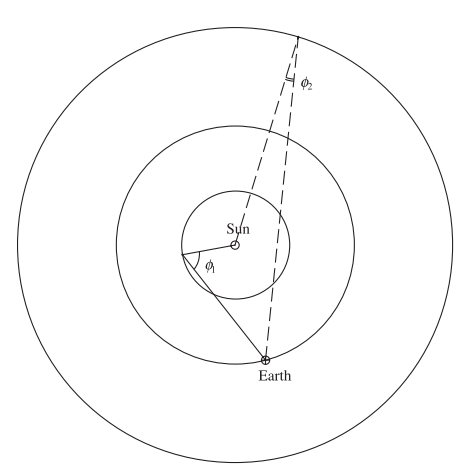
\includegraphics[width=0.4\textwidth]{images/albedo_sol_reflejo.png}
    \caption{Dispersión de la luz por un cuerpo que está iluminado por el Sol, con la radiación recibida en la 
    Tierra. En el caso de la radiación retro dispersada pura, el ángulo de fase $\phi = 0$; En el caso de la luz 
    dispersa hacia delante, $\phi= 180^\circ$ . Se indican dos planetas: uno dentro de la órbita de la Tierra, 
    con ángulo de fase $\phi1$, y otro fuera de la órbita de la Tierra, con ángulo de fase $\phi2$.
    Fuente: tomado de Fundamental Planetary Science, Jack J. Lissauer.}
    \label{fig:albedo_Reflejo}
\end{figure}
El valor del albedo varía de 0 a 1. El valor de 0 se refiere a un cuerpo negro, un medio teórico que absorbe el 
100\% de la radiación incidente. Un albedo que varía de 0.1 a 0.2 se refiere a superficies de suelo oscuras y rugosas, 
mientras que los valores alrededor de 0.4 a 0.5 representan superficies de suelo lisas y claras. El albedo de la 
cubierta de nieve, especialmente la nieve fresca y profunda, puede alcanzar hasta 0.9. El valor de 1 se refiere a 
una superficie reflectora ideal. El albedo medio del sistema Tierra es de 0.36 aproximadamente mientras qeu el de la Luna 
se encuentra cerca de 0.11 \parencite{wang2020atmosphere}
\begin{figure}[H]
    \centering
    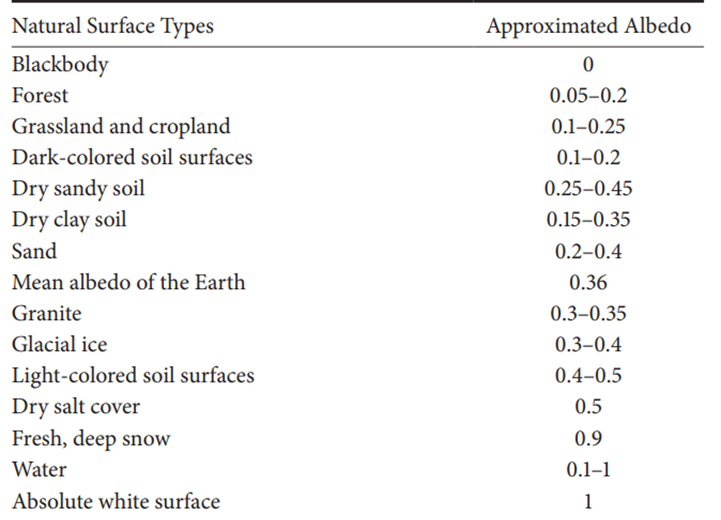
\includegraphics[width=0.5\textwidth]{images/Albedo.png}
    \caption{Valores típicos de albedo para superficies naturales.
    Fuente: tomado de Wang, Yeqiao, ed. Atmosphere and climate. CRC Press, 2020.}
    \label{fig:albedo_valores}
\end{figure}


\subsection{Emisión en Infrarrojo}\label{sec:emision_IR}
Las mediciones en el infrarrojo térmico de asteroides, satélites y cuerpos menores distantes 
son cruciales para deducir el tamaño de los objetos, sus albedos
y, en algunos casos, también las propiedades termo físicas del material de la superficie. 
Dependiendo de las mediciones disponibles y de los datos auxiliares
auxiliares disponibles, como curvas de luz visuales, información sobre el espín y la forma, 
o mediciones directas del tamaño a partir de ocultaciones o técnicas de imagen de alta 
resolución, se puede realizar una serie de cálculos simples a complejos.
de alta resolución, se aplican modelos térmicos simples o complejos para alcanzar objetivos 
científicos específicos. Sin embargo, probar estos modelos
suele ser un proceso difícil y las incertidumbres de los parámetros derivados no son fáciles 
de estimar. Aquí, hacemos un intento de verificar un modelo termo físico (TPM) ampliamente 
aceptado frente a mediciones únicas de infrarrojo térmico (IR), de disco completo y bien 
calibradas de la de la Luna. Los datos fueron obtenidos por los instrumentos High-resolution 
InfraRed Sounder (HIRS) a bordo de una flota de satélites meteorológicos de la Tierra que, 
por casualidad, se instalaron en la Luna. Encontramos 22 intrusiones lunares, tomadas en 
19 canales entre 3,75 micronm y 15,0 micronm, y en un amplio rango de ángulos de fase desde -73,1◦ 
(Luna creciente) hasta +73,8◦ (Luna menguante). Estas mediciones incluyen la Luna entera 
en un solo píxel, vista casi simultáneamente en todas las bandas. Los filtros HIRS son 
estrechos y están fuera del régimen de longitudes de onda de la característica Christiansen. 
La similitud entre estos datos lunares y las distribuciones de energía espectral-IR típicas 
de los asteroides nos permite comparar los conceptos del TPM y señalar los aspectos 
problemáticos. Las predicciones del TPM coinciden con las mediciones del HIRS en un 5
(10 \% en las longitudes de onda más cortas por debajo de 5 micronm) cuando se utilizan las 
propiedades conocidas de la Luna (tamaño, forma, espín, albedo, inercia térmica, rugosidad) 
en combinación con una emisividad hemisférica dependiente de la longitud de onda 
recientemente establecida. En los rangos de 5-7,5 micronm y 9,5- 11 micronm, el modelo de emisividad 
global se desvía considerablemente de los espectros de muestras lunares conocidos. 
Nuestros hallazgos influirán en los estudios radiométricos de asteroides cercanos a la 
Tierra y del cinturón principal en los casos en los que sólo se disponga de datos de longitud 
de onda corta (de, por ejemplo, NEOWISE, la misión warm Spitzer, o mediciones terrestres en 
banda M). El nuevo modelo lunar IR de disco completo también se utilizará para la calibración 
de instrumentos IR en misiones interplanetarias (por ejemplo, para Hayabusa-2) y satélites 
meteorológicos.
La espectroscopía de emisión térmica (en el infrarrojo a 4-25 \textmu m) se puede utilizar 
para estimar la composición mineralógica y, por lo tanto, la composición química total de rocas 
y minerales. La técnica se basa en el hecho de que los materiales emiten radiación térmica a 
frecuencias o longitudes de onda que están regidas por la geometría molecular y de red y las 
constantes de fuerza entre átomos. La emisividad espectral de un material contiene información 
que puede ser descifrada en términos de composición molecular y cristalinidad [Farmer, 1974]. 
Por lo tanto, la espectroscopía de emisión térmica es una técnica de teledetección potencialmente 
útil para mapear las composiciones en las superficies planetarias. Aquí revisamos y evaluamos 
esta técnica de teledetección para su aplicación en la exploración lunar. En particular, 
evaluamos la viabilidad de la espectroscopía de emisión térmica como una técnica efectiva para 
mapear la composición mineral y rocosa de la superficie lunar desde una nave espacial en órbita. 
El trasfondo de este esfuerzo es que un Espectrómetro de Emisión Térmica (TES) fue respaldado por 
la NASA para la exploración de Marte, y es parte de la carga útil científica en la nave espacial 
Mars Observer (MO) [Christensen et al., 1985, 1992]. TES está diseñado para llevar a cabo una 
misión de mapeo orbital no tripulado de Marte a partir de finales de 1993. La principal preocupación 
para el uso de la espectrometría de emisión IR en la Luna es el efecto bien conocido del tamaño de 
partícula en las características espectrales infrarrojas de los materiales rocosos [Lyon, 1964]. 
Es decir, la dispersión de fotones en muestras de partículas finas reduce en gran medida el contraste 
espectral de las bandas fundamentales de vibración molecular en el infrarrojo que tradicionalmente 
se han utilizado en el laboratorio para determinar la composición, lo que hace necesario que las 
aplicaciones de campo o de teledetección utilicen otras características espectrales, como la 
frecuencia de Christiansen (discutida a continuación), que no son tan conocidas. Contribuyendo a 
esta preocupación está un sentido comúnmente expresado de duda sobre la espectroscopía de emisión 
térmica para aplicaciones lunares que ha prevalecido desde finales de la década de 1960. Esta duda 
surgió de discrepancias reales o percibidas en resultados publicados donde se utilizaron técnicas de 
infrarrojo medio para observar la Luna con telescopios terrestres [por ejemplo, Goetz, 1968; Murcray 
et al., 1970; Salisbury et al., 1970; Potter y Morgan, 1981; Tyler et al., 1988; Lucey y Hawke, 1989; 
Lucey et al., 1989] y para examinar muestras lunares en el laboratorio [por ejemplo, Estep et al., 
1971; Salisbury et al., 1973; Aronson et al., 1979]. Este informe revisa las propiedades y 
procesos espectroscópicamente importantes de la superficie lunar y describe cómo la técnica 
de espectroscopía de emisión térmica se puede aplicar a la exploración lunar. Revisiones generales 
de la espectroscopia IR de minerales y polvos de roca se pueden encontrar en otros lugares de la 
literatura [por ejemplo, Farmer, 1974; Salisbury y Walter, 1989] \parencite{NAsh_douglas}.
\begin{figure}[H]
    \centering
    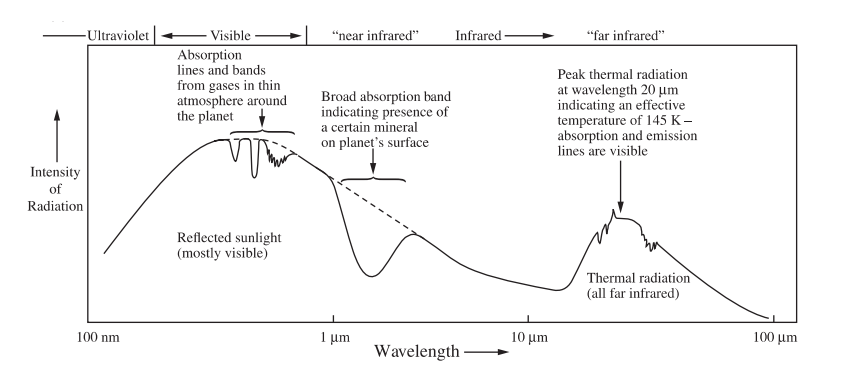
\includegraphics[width=1\textwidth]{images/Emision_moon_example.png}
    \caption{Ejemplo de un espectro de un planeta hipotético con una temperatura efectiva de 145 K. 
    El espectro se muestra desde longitudes de onda ultravioleta hasta infrarrojo lejano. 
    En las longitudes de onda más cortas, se muestra el espectro reflejado del Sol. La línea 
    discontinua muestra el espectro si no hubiera líneas ni bandas de absorción. El espectro ya 
    está corregido por el espectro de líneas de Fraunhofer del Sol. En longitudes de onda infrarrojas, 
    se detecta la emisión térmica del planeta, donde pueden estar presentes tanto líneas de absorción 
    como de emisión. Tenga en cuenta la estructura hiperfina de las bandas moleculares.
    Fuente: tomado de Hartmann 1989.}
    \label{fig:ejemplo_emision_luna}
\end{figure}
Los espectros de reflectancia, una herramienta importante para explorar la Luna, están disponibles 
en forma de mediciones de laboratorio de muestras lunares (por ejemplo, Pieters et al., 2000), 
mediciones remotas desde telescopios basados en la Tierra (por ejemplo, McCord et al., 1981; 
Lucey et al., 1986; Shkuratov et al., 2001; Kieffer y Stone, 2005; Saiki et al., 2008; Velikodsky et al., 2011) 
o naves espaciales (por ejemplo, Hillier et al., 1999; Besse et al., 2013; Wu et al., 2013; 
Ohtake et al., 2010; Boyd et al., 2012; Mahanti et al., 2016). Estas mediciones están limitadas
en su representación de la reflectancia absoluta real de la Luna debido a la perturbación 
del regolito lunar devuelto 
y la falta de un dispositivo de calibración a bordo. Los espectros de reflectancia recolectados 
in situ con un panel de calibración no solo pueden cuantificar la reflectancia absoluta, 
sino que también tienen el potencial de proporcionar más detalles composicionales y 
proporcionar una verdad de base para los datos de teledetección. 
Más singularmente, dichos datos pueden proporcionar información clave sobre el intemperismo 
espacial al medir el regolito superior no perturbado 
así como ubicaciones que han sido afectadas por el escape de cohetes de la nave espacial. 
Los primeros espectros de reflectancia in situ no se midieron hasta finales de 2013, cuando 
la nave espacial Chang'E-3 (CE-3) de China aterrizó en la Luna. 
A las 13:11:18 UTC del 14 de diciembre de 2013, CE-3 aterrizó en el norte de Mare Imbrium 
con el sitio de aterrizaje en 
(44.1281°N, 19.5110°W). El sitio de aterrizaje está a unos 50 m al este de un cráter de 450 m 
llamado Zi Wei. 
La unidad del sitio de aterrizaje pertenece a la última fase importante del vulcanismo lunar 
(basaltos del Eratosteniano) con una edad recién fechada de aproximadamente 2.35 Ga (Wu et al., 2015). 
Estos basaltos no muestreados atrajeron una atención significativa hace bastante tiempo debido a 
su edad relativamente joven y espectros únicos en términos de oscuridad, color azul, absorción de 
1  micron amplia y absorción atenuada de 2 micron (por ejemplo, Staid et al., 2011; Wu et al., 2015). 
Un espectrómetro Visible-Cercano Infrarrojo (VNIS) fue llevado en el rover “Yutu (Conejo de Jade)” 
y midió el primer conjunto de espectros de reflectancia in situ de la Luna. 
Los primeros trabajos sobre VNIS se centraron principalmente en la descripción/calibración instrumental 
(He et al., 2014; Xu et al., 2014; Liu et al., 2014) o análisis mineral y elemental 
(Zhang et al., 2015a, 2015b; Ling et al., 2015; Hu et al., 2015; Wang et al., 2017) \parencite{McCord}.\\
\\
Salisbury, Basu y Fisher realizaron mediciones de los espectros de reflectancia hemisférica 
direccional en el 
infrarrojo (2.08–14 $\mu$m) de los suelos lunares que representan las 
principales unidades litológicas muestreadas hasta ahora en la superficie 
lunar, y de suelos con diferentes edades de exposición dentro de esas 
unidades. Tales espectros de reflectancia (R) pueden utilizarse para 
calcular la emisividad absoluta (E) usando la Ley de Kirchhoff (E = 1 - R). 
Los efectos de la edad de exposición varían según la región del espectro. 
En las regiones de 2–5 $\mu$m y 8–14 $\mu$m, los suelos lunares se oscurecen 
con la edad de exposición, consistente con el comportamiento espectral en el 
VNIR y el efecto óptico dominante de cantidades crecientes de hierro metálico 
finamente dividido en suelos más maduros. Sin embargo, en la región de 5–8 
$\mu$m los suelos tienden a mostrar mayores reflectancias con una mayor edad 
de exposición, lo que sugiere algún cambio no anticipado en las propiedades 
ópticas del hierro metálico fino en esas longitudes de onda. La característica 
espectral más útil para la teledetección composicional es el mínimo de 
reflectancia de Christiansen (máximo de emisividad), cuyo contraste espectral 
es realzado por el ambiente lunar, y cuya posición en la longitud de onda puede 
relacionarse con la composición sin verse mucho afectada por la edad de 
exposición. El ambiente de vacío en la superficie lunar no solo mejora el 
contraste espectral de la característica de Christiansen, sino que también lo 
desplaza ligeramente a longitudes de onda más cortas, un efecto que debe ser 
compensado al inferir la composición. En contraste con la característica de 
Christiansen, las débiles y relativamente pocas bandas de absorción 
en la región de dispersión de volumen entre 3 y 8 $\mu$m 
parecen ser de utilidad limitada. Las bandas de reststrahlen también son muy 
débiles en los espectros de emisividad absoluta, y evidentemente no son mejoradas 
por el ambiente lunar de la misma manera que la característica de Christiansen. 
Así, solo pueden ser utilizadas para la teledetección con mediciones de una 
señal-ruido extraordinariamente alta (1000/1). Sin embargo, estas características, 
así como la característica de transparencia (que es particularmente prominente en 
los espectros de suelos feldespáticos), contienen importante información 
mineralógica, como las abundancias relativas de plagioclasa y piroxeno, y pueden 
ser utilizadas para estudios de laboratorio de suelos lunares. Análisis 
mineralógicos más ciertos y cuantitativos de los suelos lunares parecen factibles 
tras análisis espectrales adicionales de separaciones de suelos, y análisis 
mineralógicos adicionales de muestras de suelos para las cuales se disponga de 
datos espectrales \parencite{SALISBURY1997125}.\\
\\
Desde los primeros días de la teledetección espectroscópica de la superficie lunar, 
las bandas de transición electrónica exhibidas por los suelos lunares en las regiones 
del espectro visible e infrarrojo cercano (VNIR) se han utilizado para determinar la 
composición mineralógica (por ejemplo, McCord y Johnson, 1970; McCord et al., 1972; 
Adams, 1974). También hubo un reconocimiento temprano de los efectos del intemperismo 
espacial en los suelos lunares y en su reflectancia espectral (por ejemplo, McKay et 
al., 1974; Hapke et al., 1975; Morris, 1976; Charette et al., 1976; y Basu, 1977), 
resultando en un modelo básico que, sin embargo, continúa refinándose (por ejemplo, 
Pieters et al., 1993; Fischer y Pieters, 1994; y Clark y Johnson, 1996). Brevemente, 
los suelos lunares se derivan principalmente de la trituración de las rocas subyacentes 
por impacto hiperveloz. Con el tiempo, una lluvia de impactos de micrometeoritos continúa 
el proceso de trituración pero, junto con la erosión del viento solar, también produce 
progresivamente más fase de fusión y vapor depositado desde vapor en las superficies de 
los granos. Aunque otros procesos afectan un suelo envejecido, son las partículas de hierro 
las que, en y sobre los granos, principalmente en aglutinados soldados por vidrio, son 
las que principalmente explican el oscurecimiento y enrojecimiento de la reflectancia del 
suelo lunar con la edad de exposición en la superficie lunar, así como la disminución del 
contraste espectral de las bandas de transición electrónica. En consecuencia, un buen 
método para relacionar la edad de exposición del suelo lunar con sus cambiantes propiedades 
ópticas es utilizar la resonancia ferromagnética para medir la intensidad de la resonancia 
característica del hierro de dominio único dentro del suelo normalizado al contenido de FeO, 
obteniendo el índice de exposición ampliamente utilizado, Is/FeO (Morris, 1976). Este enfoque 
fue utilizado por Fischer (1995) para seleccionar conjuntos de suelos lunares de composición 
similar pero diferentes edades de exposición para estudiar el efecto del intemperismo espacial 
lunar en los espectros de reflectancia.

\subsection{Coordenadas Selenográficas}
La Unión Astronómica Nacional (IAU), ha establecido un sistema de referencia de coordenadas para los distintos cuerpos del sistema solar.
En la Tabla \ref{tab:IAU_coor}, se muestra una lista de estos sistemas de coordenadas aceptados.
\begin{table}[H]
    \centering
    \caption{Sistemas de Coordenadas aceptados por la IAU para planetas y satélites}
      \begin{tabular}{|p{4.215em}|p{14.355em}|p{11.93em}|}
      \toprule
      \multicolumn{1}{|c|}{Cuerpo} & \multicolumn{1}{c|}{Sistema de Coordenadas} & \multicolumn{1}{c|}{Red de Control} \\
      \midrule
      \textcolor[rgb]{ .106,  .106,  .106}{Io} & \textcolor[rgb]{ .106,  .106,  .106}{Planetographic, +West, 0 - 360} & \textcolor[rgb]{ .106,  .106,  .106}{Voyager/Galileo SSI} \\
      \midrule
      \multirow{2}[4]{*}{\textcolor[rgb]{ .106,  .106,  .106}{Mars}} & \textcolor[rgb]{ .106,  .106,  .106}{Planetocentric, +East, 0 - 360} & \textcolor[rgb]{ .106,  .106,  .106}{MDIM 2.0} \\
  \cmidrule{2-3}    \multicolumn{1}{|c|}{} & \textcolor[rgb]{ .106,  .106,  .106}{Planetographic, +West, 0 - 360} & \textcolor[rgb]{ .106,  .106,  .106}{MDIM 2.1} \\
      \midrule
      \multirow{2}[4]{*}{\textcolor[rgb]{ .106,  .106,  .106}{Moon}} & \multirow{2}[4]{*}{\textcolor[rgb]{ .106,  .106,  .106}{Planetographic, +East, -180 - 180}} & \textcolor[rgb]{ .106,  .106,  .106}{ULCN 2005} \\
  \cmidrule{3-3}    \multicolumn{1}{|c|}{} & \multicolumn{1}{c|}{} & \textcolor[rgb]{ .106,  .106,  .106}{LOLA 2011} \\
      \midrule
      \multirow{2}[4]{*}{\textcolor[rgb]{ .106,  .106,  .106}{Mercury}} & \multirow{2}[4]{*}{\textcolor[rgb]{ .106,  .106,  .106}{Planetographic, +West, 0 - 360}} & \textcolor[rgb]{ .106,  .106,  .106}{Preliminary MESSENGER} \\
  \cmidrule{3-3}    \multicolumn{1}{|c|}{} & \multicolumn{1}{c|}{} & \textcolor[rgb]{ .106,  .106,  .106}{MESSENGER Team} \\
      \midrule
      \textcolor[rgb]{ .106,  .106,  .106}{Pluto} & \textcolor[rgb]{ .106,  .106,  .106}{Planetocentric, +East, 0 - 360} & \textcolor[rgb]{ .106,  .106,  .106}{Pluto} \\
      \bottomrule
      \end{tabular}%
    \label{tab:IAU_coor}%
\end{table}%
Una red de control está compuesta por una red de puntos de control. Un punto de control es una ubicación en un planeta 
o satélite que se utiliza como referencia. Un conjunto de puntos de control en una red de control nos permite calcular 
con precisión la ubicación de una característica en un planeta o satélite en relación con la red de puntos de control 
que se encuentran en la red de control.\\
\\
Puede haber numerosas redes de control para un cuerpo planetario porque a medida que se obtienen datos más precisos, 
la ubicación de los puntos de control cambia, y todas las características que tienen sus ubicaciones definidas en 
relación con una red de control particular deben actualizarse para reflejar su nueva ubicación en relación con los 
nuevos datos.\\
\\
Todos los cuerpos planetarios actualmente en la base de datos de nomenclatura, excepto Marte, se definen como una esfera, 
incluso si el cuerpo no es muy esférico. Para los cuerpos triaxiales, la IAU define una esfera de mejor ajuste para 
aproximar la forma para aplicaciones cartográficas. Un beneficio de usar una esfera es que una latitud planetocéntrica 
y planetográfica definida será la misma. Sin embargo, para Marte, que se define como una elipse (biaxial), los dos 
sistemas de latitud son realmente diferentes.\\
\\
Una latitud planetocéntrica se define como el ángulo entre el plano ecuatorial y una línea desde el centro del cuerpo. 
La latitud planetográfica es el ángulo entre el plano ecuatorial y una línea que es normal al cuerpo. Ambas latitudes 
son equivalentes en un modelo esférico, pero pueden diferir considerablemente en un elipsoide \parencite{iau_control_networks}.\\
\subsubsection{Coordenadas Planetocéntricas}
Estas son coordenadas esféricas 
dextral donde el eje "z" es el eje medio de rotación y el eje x es la intersección del ecuador y el 
meridiano principal. El eje "x" es normal al eje z a través del origen del sistema, que es el 
centro de masa de la Luna. El eje "y" es ortogonal a los ejes "x" y "z". La latitud es el ángulo entre una 
línea que se extiende desde el origen hasta el ecuador planetario y un vector desde el origen hasta el punto de 
interés. La longitud es el ángulo entre este vector y el plano del meridiano principal medido en 
una dirección oriental. El radio es la distancia desde el centro de masa de la Luna hasta el punto de interés \parencite{lro_coordinate_system} 
Las coordenadas planetocéntricas se ilustran en la Figura \ref{fig:coordenadas_luna}.
\begin{figure}[H]
    \centering
    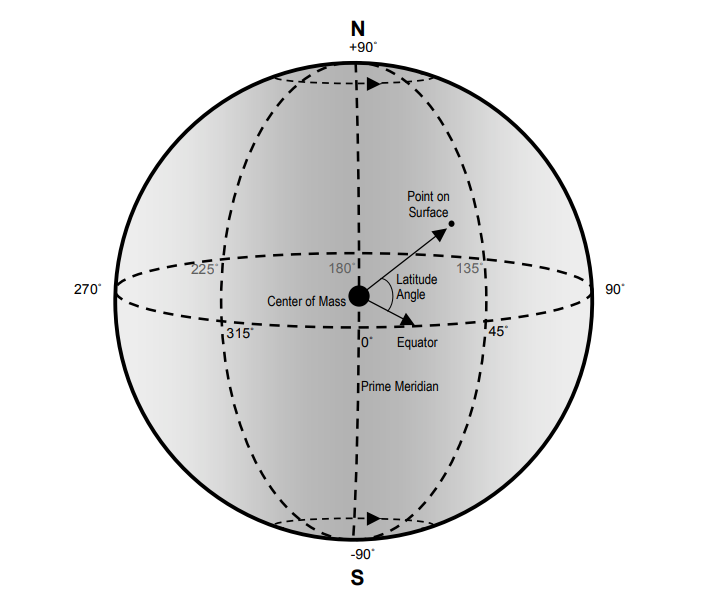
\includegraphics[width=0.6\textwidth]{images/coord_planetocentricas.png}
    \caption{Las coordenadas planetocéntricas se expresan con el origen en el centro de masa del cuerpo. Fuente: tomado de pds-imaging.jpl.nasa.gov}
    \label{fig:coordenadas_luna}
\end{figure}

El radio debe expresarse como la distancia total desde el centro de masa de la Luna hasta 
el punto de interés. Si es necesario, por ejemplo, para evitar el error de redondeo en un modelo de terreno digital 
grande en formato de 4 bytes, la distancia de un punto desde el centro de masa de la Luna se puede expresar como la 
distancia a lo largo del vector de radio por encima (positivo) o por debajo (negativo) de una esfera de referencia de radio 
1737.4 km (el valor del Informe del Grupo de Trabajo de la IAU/IAG sobre Coordenadas Cartográficas y Elementos Rotacionales 
del año 2000). El radio de la esfera de referencia dado debe utilizarse hasta que algún valor actualizado sea 
aceptado internacionalmente, por ejemplo, después de la misión LRO \parencite{lro_coordinate_system}.

\subsection{La Luna}
Actualmente la teoría mas aceptada en general sobre la formación de la Luna es que la Luna comenzó 
como un pequeño planeta rocoso, a veces llamado Theia (la diosa) en honor a Theia Euryphaessa, l
a madre de Selene (la diosa de la Luna) en la mitología griega. Originalmente en una órbita cercana 
a lo que ahora es el cinturón de asteroides, la interacción con otros cuerpos perturbó esa órbita y 
dirigió a Theia hacia el Sol. En el camino, encontró a la Tierra, golpeándola de refilón y vaporizando, 
fundiendo y pulverizando a Theia y parte de la corteza terrestre. La Luna se formó a partir de la parte 
de la nube resultante que orbitaba la Tierra. Parte de la evidencia de esto es la deficiencia de materiales 
volátiles como el agua y los sulfuros en la Luna; debieron quedarse en la nube y dispersarse en el espacio o 
regresar a la Tierra \parencite{byrne2008far}.\\
\\
A medida que la Luna se fue formando, habría constituido un cuerpo muy caliente y fundido, casi esférico 
pero ligeramente oblato debido a su rotación, y quizás distorsionado adicionalmente por la proximidad de la 
gravedad de la Tierra. La mezcla fundida de elementos que existía en este tiempo temprano, hace 4 mil millones 
de años, se llama el Océano de Magma. A medida que el Océano de Magma se enfriaba, los compuestos más pesados 
se desplazaron hacia el núcleo y los más ligeros subieron hacia la superficie. Algunos de los elementos 
más pesados y comunes, como el hierro, quizás en combinación con algo de azufre, se asentaron en el núcleo. 
Los elementos más ligeros, especialmente el silicio y el oxígeno en forma de silicatos de metales como el aluminio, 
comenzaron a formar una corteza que estableció una discontinuidad en la densidad similar a la que existe entre 
la corteza de la Tierra y su manto. En la Tierra, ese límite se llama la discontinuidad de Mohorovičić 
\parencite{Origin_of_the_moon}\parencite{byrne2008far}.\\
\\
El lado lejano de la Luna es el lado que no podemos ver desde la Tierra. Debido a que la rotación de 
la Luna tiene un acoplamiento de marea en sincronía mientras gira alrededor de la Tierra, su lado cercano siempre 
mira hacia la Tierra. Si las personas vivieran en la Luna, aquellos que vivieran en el lado cercano 
siempre verían la Tierra y aquellos que vivieran en el lado lejano nunca la verían.
Esta situación (que es común a las grandes lunas de todos los planetas) ha llevado a un aura de 
misterio sobre el lado lejano de la Luna desde que los humanos pensaron en la iluminación nocturna. 
Cuando la humanidad pensaba que estaba en el centro del universo, esta condición parecía lo 
suficientemente natural, pero cuando prevaleció la visión copernicana del sistema solar, hubo un 
período en el que la gente se preguntaba cómo sería el lado lejano.¿Había un patrón allí como el del 
lado cercano? ¿Era completamente diferente? ¿Estaba coloreado, como Marte, o casi sin color como el 
lado cercano? ¿Había mares y océanos, como una vez se pensó que había en el lado cercano?
El lado cercano de la Luna es un símbolo de romance. El lado lejano a menudo ha sido llamado el 
lado oscuro de la Luna, como si nuestra incapacidad para verlo significara que nunca estaba iluminado, a pesar
que recibe tanta luz solar como el lado cercano. Cuando las sondas espaciales Luna 3, Zond 3 y Lunar Orbiter 
1 transmitieron imágenes de vuelta a la Tierra, se hizo evidente que la naturaleza del 
lado lejano de la Luna era realmente muy diferente a la del lado cercano \parencite{byrne2008far}.

\subsubsection{Topografía Lunar}
En relacion con el relieve de la Luna se dispone de una gran cantidad de datos, expresados en los 
libros de Elger, Neison, Nasmyth y Carpenter, 
Shaler, Graff, Fisher y otros, así como en 
las magníficas fotografías de la Luna tomadas 
en los observatorios de París, Lick y Mount Wilson. 
De valor único es el suntuoso atlas lunar 
de Loewy y Puiseux, que representa una 
docena de años de estudio fotográfico en el Observatorio de París. 
Los antiguos mapas dibujados a mano 
de Baer y Maedler, Schmidt y otros son 
históricamente importantes y de valor permanente, 
pero para muchos propósitos no son tan útiles como las 
fotografías. La siguiente discusión se 
confinará en gran medida a los llamados "cráteres", 
rayados y no rayados, y los mares. 

Según la explicación favorecida 
del origen de la Luna, su material silicatado 
estaba inicialmente lo suficientemente caliente como para ser líquido en 
la superficie y contenía mucho gas disuelto; que 
había algo de gas libre presente en los fragmentos terrestres; 
y que más tarde probablemente se liberó gas adicional por la cristalización a presión de 
silicato en las profundidades del globo lunar. 
Por lo tanto, es natural buscar signos de acción volcánica moderada 
en la topografía de la Luna. De 
hecho, ninguna otra explicación parece tan plausible para 
ciertas filas de pequeños pozos alineados, tipificados por 
los que se encuentran en las cercanías de los "cráteres" Bulliadus y Stadius. 
Tales supuestos cráteres verdaderos, comparativamente pequeños, deben contarse por 
decenas si no por cientos; sin embargo, su área total es 
solo una pequeña fracción de la superficie visible de la 
Luna. 

Muchos selenógrafos se han inclinado a 
aceptar un origen similar para los miles de 
depresiones mucho mayores: llanuras amuralladas, anillos montañosos, 
llanuras craterizadas y "cráteres" de la clasificación de Neison. 
Para esta conclusión hay pocos argumentos 
convincentes. En su apoyo se ha hecho hincapié 
en una supuesta homologación con las 
depresiones terrestres mayores debidas a explosiones volcánicas importantes, 
y también con los sumideros volcánicos 
(desafortunadamente llamados "calderas") de 
Hawái. 

La primera de estas pretensiones de verdadera homologación es 
sospechosa en cuanto se compara la 
asimetría característica en los planos de estas "calderas" 
terrestres de evisceración con el alto grado de simetría de las depresiones 
lunares. Otros contrastes se encuentran en la gran 
disparidad de tamaño, en la abundancia relativa, y en la 
distribución sobre las respectivas superficies de 
planeta y satélite. En ninguno de estos aspectos 
el vulcanismo de tipo explosivo es una buena 
explicación para los muchos miles de "cráteres" más grandes. 

La sugerencia de J. D. Dana (1846), seguida 
por la de W. H. Pickering (1906), de que 
los sumideros hawaianos pueden representar más verdaderamente las 
depresiones anilladas de la Luna también es 
insatisfactoria. Los sumideros hawaianos son efectos superficiales 
de hundimientos, causados en gran parte por el 
retiro de lava a través de fisuras que se han 
abierto en el poderoso domo de lava de Hawái, este 
retiro es posible porque la gran 
elevación del domo visible sobre el 
suelo del Pacífico proporciona la condición requerida para el 
drenaje de lava de las tuberías o 
conductos activos. En la Luna no existe tal diferencia 
de nivel para inducir un retiro importante de lava 
en profundidad \parencite{Reginaldb}.
\subsubsection{Temperatura de la Luna}
Dado que la latitud subsolar en la Luna no excede los 1.6◦, las partes 
internas de algunos cráteres en las regiones polares lunares permanecen en sombra 
durante todo el año, formando regiones permanentemente sombreadas (PSR). 
Los PSR pueden mantener temperaturas extremadamente bajas durante mucho tiempo, creando 
condiciones favorables para el almacenamiento de hielo de agua.\\
\\
La inclinación del eje de rotación lunar provoca cambios de temperatura estacionales 
en las regiones polares lunares. La acumulación de datos observacionales a largo plazo 
de Diviner permite el estudio de variaciones de temperatura estacionales. Williams et al. 
(2019) mapearon las temperaturas estacionales en regiones con latitudes mayores de 80◦, 7
y encontraron que 
el ciclo térmico en las PSR tenía variaciones estacionales significativas. Liu y Jin 
(2019) presentaron el modelo de simulación de temperatura estacional de no PSR cerca de 
los polos lunares con la posición subsolar en tiempo real. Liu y 
Jin (2020) tomaron el PSR en el cráter Hermite-A en el polo norte como un 
ejemplo para estudiar las variaciones de temperatura diurnas y estacionales en 
las PSR. La emisividad y la conductividad térmica en el PSR fueron 
analizadas con los datos de Diviner.\\
\\
Las principales fuentes de calor de un PSR son la radiación térmica y la luz solar dispersa, 
que son diferentes del caso de los no PSR. La mayoría de los estudios previos 
se han centrado en regiones de baja latitud con altas temperaturas, y hay una falta de 
investigación sobre los parámetros termofísicos de los PSR 
en entornos de temperatura extremadamente baja. En 2019, Woods-Robinson 
et al. (2019) sugirieron que los parámetros termofísicos ampliamente utilizados 
para no PSR no son adecuados para temperaturas por debajo de 100 K. Propusieron un 
modelo derivado de la física del estado sólido y mediciones de simulantes lunares 
para la capacidad calorífica y la conductividad térmica del regolito bajo temperaturas 
extremadamente bajas. Sin embargo, este modelo de conductividad térmica 
difiere a altas temperaturas del modelo comúnmente utilizado de Hayne 
et al. (2017). Martinez y Siegler (2021) propusieron un nuevo modelo de 
conductividad térmica adecuado tanto para entornos de temperatura extremadamente baja 
en PSR como para entornos de alta temperatura expuestos a la luz solar directa. 
Pero el nuevo modelo carece de validación por observaciones de teledetección \parencite{Zhengling2024}.\\

\section{Metodología}\label{sec:metodologia}
El proyecto se desarrollara en distintas fases atendiendo al alcance de cada uno de los 
objetivos específicos y el objetivo general, en ese sentido se plantea la siguiente metodología:
\begin{itemize}
    \item El primer paso será una caracterización cualitativa por medio de una 
    revisión bibliográfica, en la revisión bibliografía se buscaran los datos disponibles de
    la mayor cantidad de misiones de exploración Lunar. Para la determinación de los parámetros y propiedades 
    principales que controlan la temperatura se deben obtener datos morfológicos, como modelos digitales de 
    superficie, composición del regolito Lunar, condiciones ambientales particulares, diferencias con el lado visible, 
    entre otros. Seguidamente se deben obtener los datos de características ópticas de la Luna, como albedo y 
    reflectancia, las mediciones hechas por los diferentes orbitadores, sondas, y rovers.Y por ultimo se obtendrán 
    los datos de la caracterización térmica, aquí se busca obtener mediciones de temperatura, emisión en el infrarrojo y
    condiciones de exposición solar, para esto se consultaran las diferentes dispositivos que han hecho mediciones sobre 
    la superficie de la Luna. El conjunto de cada uno de los datos obtenidos, generara el listado completo de parámetros 
    principales de la caracterización de la región que contiene a los cráteres Garavito.
    \item A partir de los datos obtenidos se buscará reproducir las condiciones de radiancia solar en la Luna, específicamente 
    en la región de los cráteres Garavito. Para esto se desarrollará el cálculo para determinar la posición 
    del Sol en el cielo local y se desarrollará un programa en lenguaje Python, además se buscaran diferentes softwares 
    de referencia que simulen condiciones locales de iluminación, con el fin de generar una comparación y verificación. 
    Con el modelo calibrado se espera poder determinar la temperatura sobre la superficie de los cráteres Garavito.
    \item Por ultimo se generarán las curvas de emisión en el óptico y infrarrojo para los diferentes momentos del día 
    lunar, en esta etapa se reunirá toda la información de la caracterización y simulaciones, para evaluar las condiciones 
    de radiancia Lunar para las condiciones visibles y térmicas.Esto se hará con ayuda de herramientas para el análisis de distribuciones
    espectrales de energía (SED) con la herramienta CIGALE \parencite{Boquien2019}. como ejercicio final se buscara hacer 
    la comparación con una región del lado visible de la Luna.
\end{itemize}

\section{Presupuesto y Fuentes de Financiación}
Debido a la metodología que se utilizará en el desarrollo del proyecto, no se requiere de un presupuesto 
propio o asignado ni de alguna fuentes de financiación adicionales para las actividades a desarrollar.

\section{Cronograma}
El cronograma, se construyo considerando un tiempo adecuado para la ejecución y cumplimiento de cada una 
de las actividades establecidas.
\begin{figure}[H]
    \centering
    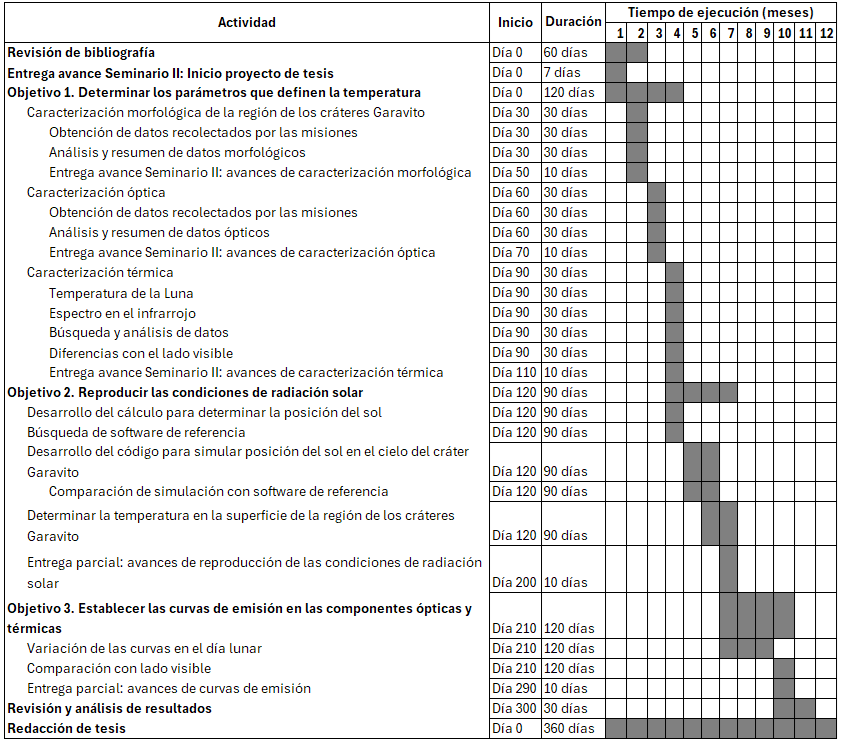
\includegraphics[width=1\textwidth]{images/Schedule.png}
    \caption{Cronograma de actividades para la ejecución del proyecto}
    \label{fig:cronograma}
\end{figure}

\newpage
\printbibliography
\end{document}